\documentclass[11pt]{article}
\usepackage[margin=1in]{geometry}
\usepackage{graphicx}
\usepackage{booktabs}
\usepackage{hyperref}
\usepackage{float}
\title{Traffic Speed Forecasting: AML Baselines and Graph Learning}
\author{Project Report}
\date{\today}
\begin{document}
\maketitle

\begin{abstract}
This project compares persistence, a segment-wise multi-output Random Forest, pooled XGBoost, and a trained Graph Attention Network (GAT) on five-minute METR-LA speed observations. Models are evaluated chronologically at 5, 15, 30, and 60 minutes. The GAT and fixed sensor graph are implemented and trained; in this run, the GAT does not outperform the tree baselines on overall MAE. The traffic CSVs contain speed only, so flow, occupancy, and signal-control simulation are not claimed.
\end{abstract}

\section{Data and graph}
METR-LA contains 34,272 timestamps for 207 sensors from March 1 to June 27, 2012. PEMS-BAY contains 52,116 timestamps for 325 sensors from January 1 to June 30, 2017. Zero speeds are treated as missing, forward-filled only for causal inputs, and excluded from target training and scoring. Flow and occupancy are not supplied.

Official METR-LA sensor IDs, locations, and road distances are sourced from DCRNN commit \texttt{602afd9d767d3aa1c9b3eac51710d6aeee12c227}. The IDs align with all 207 METR-LA traffic columns. A Gaussian distance kernel and threshold of 0.1 produce a symmetrized 207-node graph with 1,313 undirected links. This graph does not encode verified upstream/downstream direction.

\IfFileExists{../results/figures/01_traffic_data_quality.png}{
\begin{figure}[H]\centering
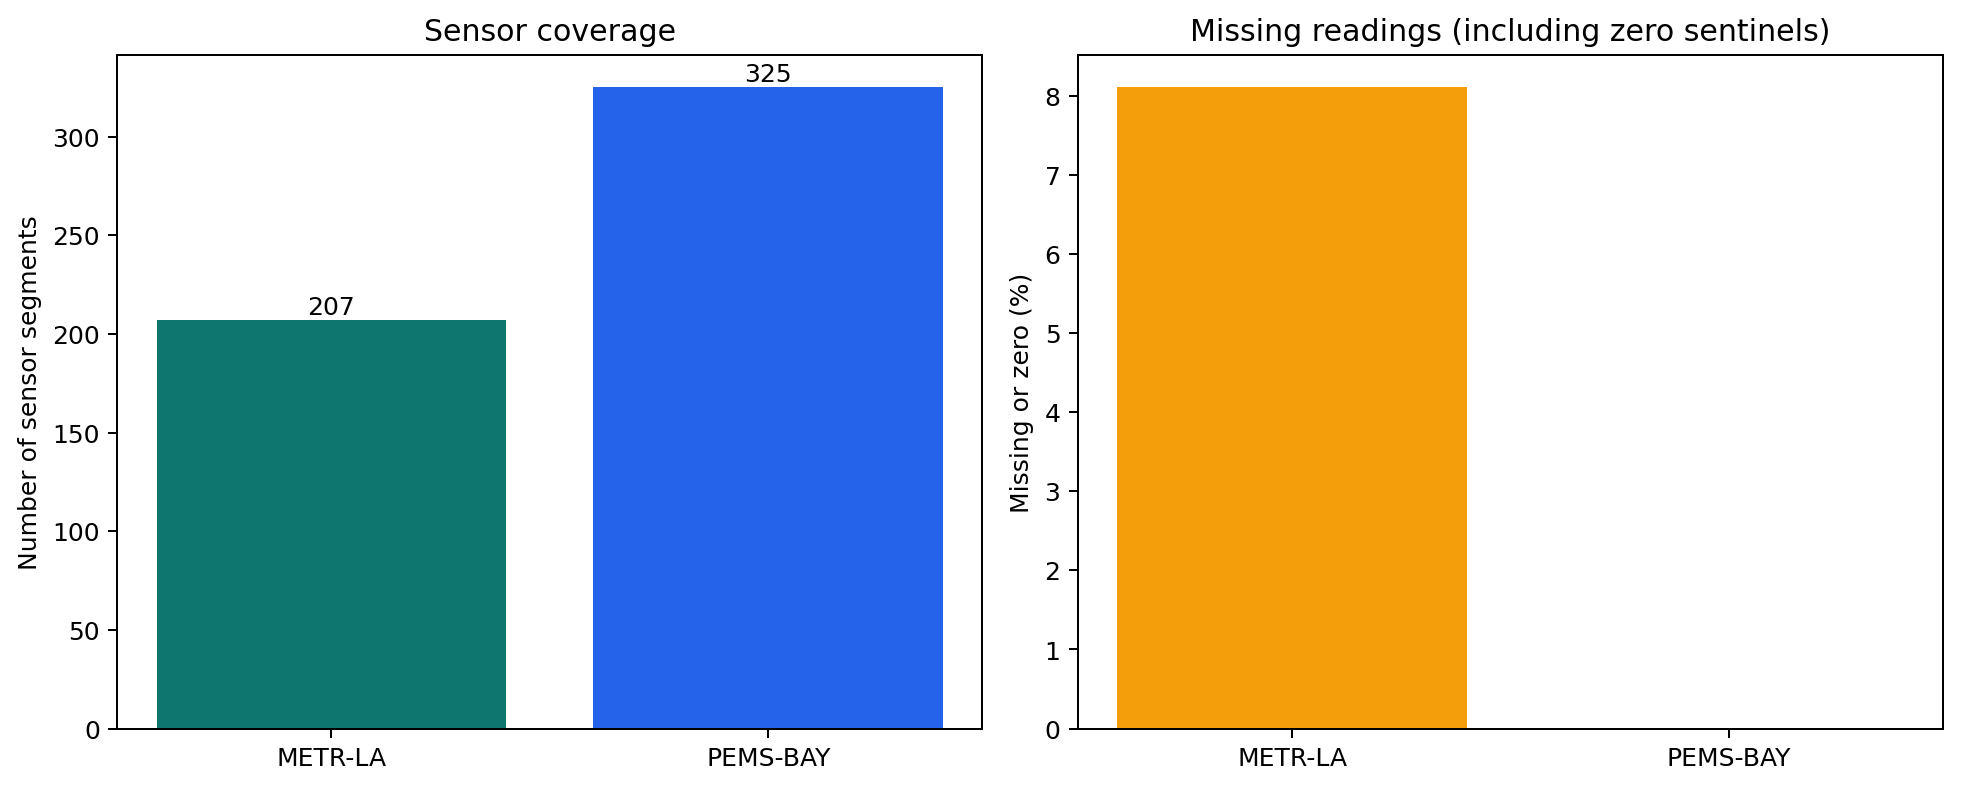
\includegraphics[width=.85\linewidth]{../results/figures/01_traffic_data_quality.png}
\caption{Traffic sensor coverage and missing readings.}
\end{figure}}{}

\section{Forecast protocol and models}
Chronological partitions are 70\% training, 10\% validation, and 20\% test. The forecast horizons are 5, 15, 30, and 60 minutes. Peak is weekdays 07:00--09:59 and 16:00--18:59; all remaining times, including weekends, are off-peak. MAE, MAPE, and RMSE are computed over observed nonzero targets only.

Persistence predicts the last observed speed. The Random Forest trains one multi-output model per sensor using causal speed lags and cyclic time features, with up to 2,000 training timestamps per sensor. Pooled XGBoost uses the same general feature family and sensor identity, with up to 50,000 observed training targets per horizon.

The GAT applies spatial attention over the fixed graph. It uses six consecutive five-minute speed observations and cyclic time/weekday features, and is trained with masked loss and validation-based early stopping. Per-sensor scaling is fit only on training timestamps. The implementation ran on MPS for six epochs; best validation masked MSE was 0.4220. All models share test origins and valid target counts and use at most 25 minutes of input history. Training volumes and exact feature representations differ, so this is not an equal-compute benchmark.

\section{Overall held-out results}
\begin{center}
\small
\begin{tabular}{llrrr}
\toprule
Horizon & Model & MAE & MAPE (\%) & RMSE \\
\midrule
5 min & Persistence & 2.814 & 6.489 & 4.627 \\
5 min & Random Forest & \textbf{2.519} & 6.327 & \textbf{4.281} \\
5 min & XGBoost & 2.554 & 6.435 & 4.326 \\
5 min & GAT & 2.879 & 7.206 & 4.511 \\
15 min & Persistence & 3.499 & 8.612 & 6.418 \\
15 min & Random Forest & \textbf{3.119} & \textbf{8.431} & \textbf{5.702} \\
15 min & XGBoost & 3.239 & 8.846 & 5.873 \\
15 min & GAT & 3.466 & 9.168 & 5.830 \\
30 min & Persistence & 4.207 & 10.858 & 8.052 \\
30 min & Random Forest & \textbf{3.635} & \textbf{10.401} & \textbf{6.706} \\
30 min & XGBoost & 3.854 & 11.106 & 6.988 \\
30 min & GAT & 4.087 & 11.434 & 6.965 \\
60 min & Persistence & 5.381 & 14.535 & 10.345 \\
60 min & Random Forest & \textbf{4.192} & \textbf{12.623} & \textbf{7.657} \\
60 min & XGBoost & 4.542 & 13.696 & 7.982 \\
60 min & GAT & 4.898 & 14.328 & 8.227 \\
\bottomrule
\end{tabular}
\end{center}

Random Forest has the lowest overall MAE at all horizons. GAT improves on persistence MAE at 15, 30, and 60 minutes, but not at 5 minutes; it remains behind both tree models overall.

\IfFileExists{../results/figures/27_metr_la_peak_offpeak_model_comparison.png}{
\begin{figure}[H]\centering
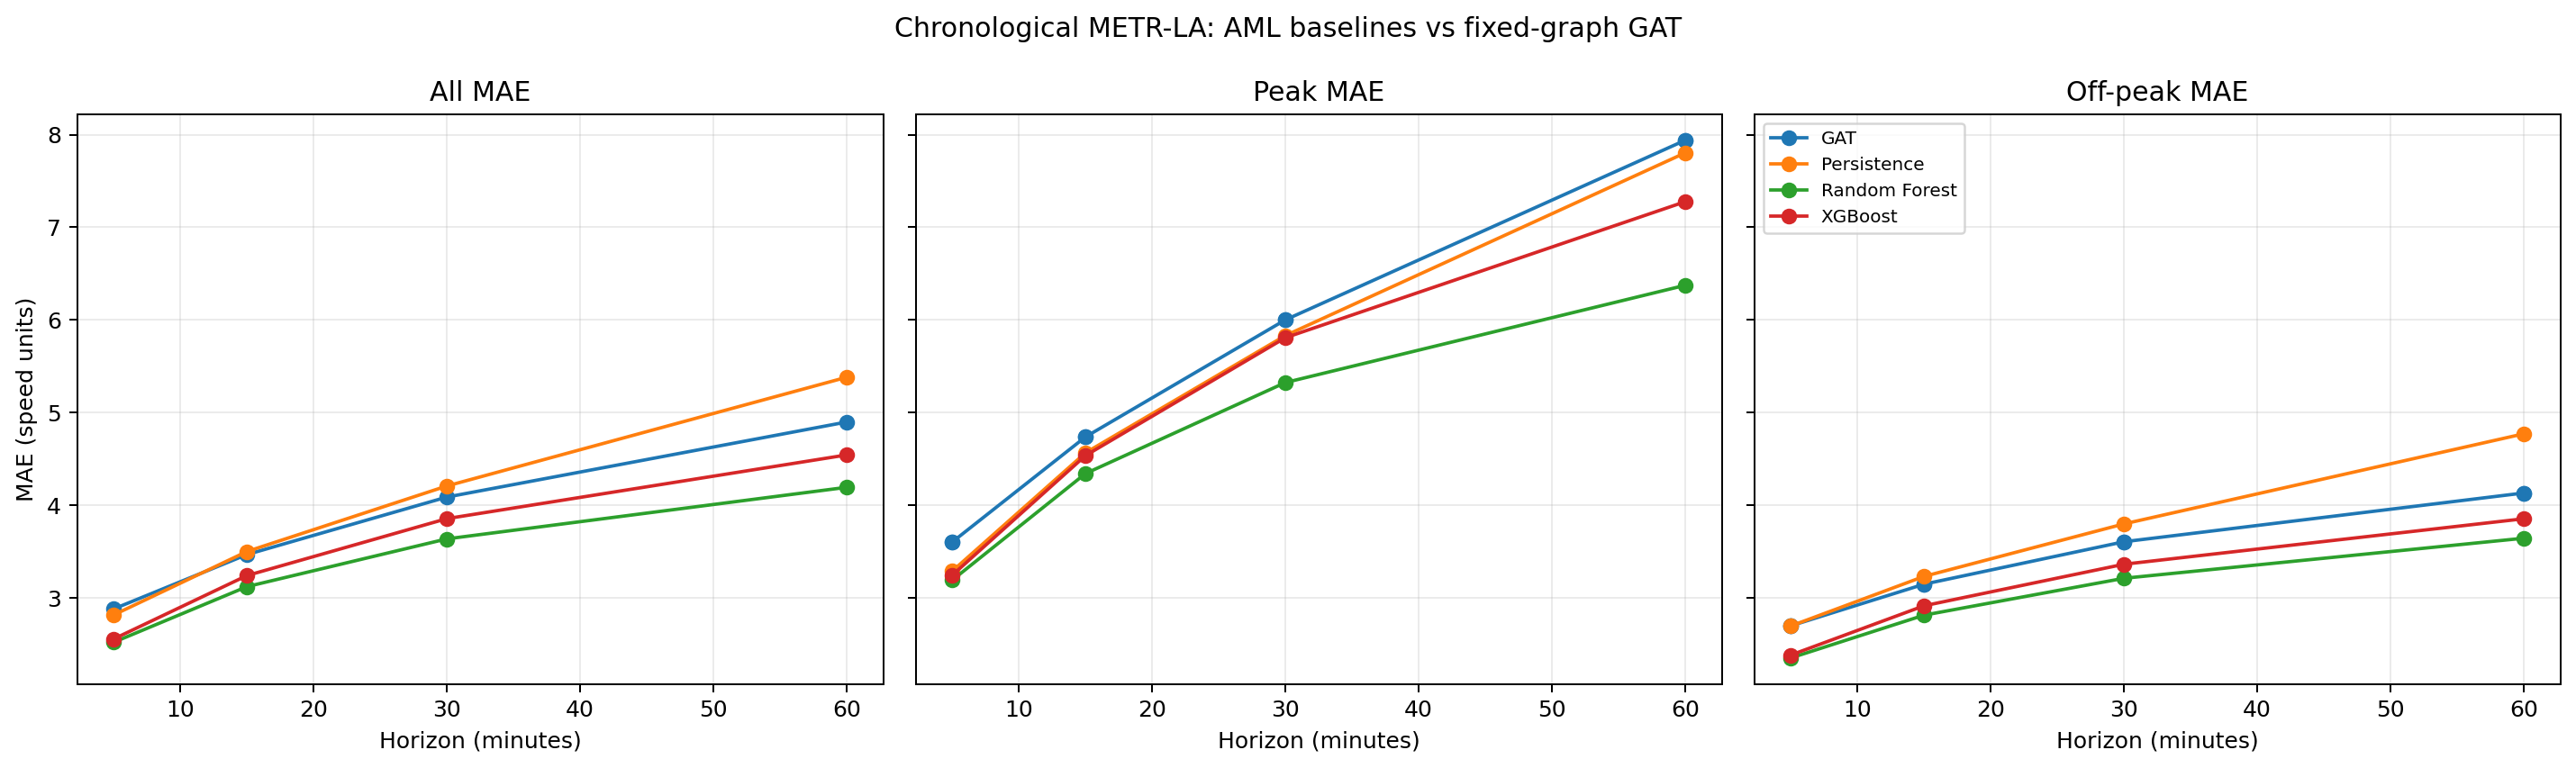
\includegraphics[width=.9\linewidth]{../results/figures/27_metr_la_peak_offpeak_model_comparison.png}
\caption{Held-out MAE by horizon for overall, weekday peak, and off-peak periods.}
\end{figure}}{}

\section{Limitations and reproducibility}
The fixed graph is symmetrized and does not encode verified travel direction. Flow/occupancy forecasting and SUMO signal simulation remain incomplete because flow/queue measurements, signal phases, and timing plans are unavailable. The supplied reference scores are not represented as reproduced project results.

Run notebooks 01--09 in order. Metrics, figures, sample forecasts, generated adjacency, and GAT state are saved under \texttt{results/}. Full overall and period-specific MAE/MAPE/RMSE tables are in \texttt{results/metrics/metr\_la\_model\_comparison.csv}.

\bibliographystyle{plain}
\bibliography{references}
\end{document}
